
\subsubsection{Sparse-Oracles for Fermionic Pairing Hamiltonian}

Liu et. al \cite{liu2024efficient} use the framework proposed by Camps et. al \cite{camps2024explicit} to construct a Sparse-Oracle block-encoding for a pairing Hamiltonian of the form:
\begin{equation}
    \label{eq:pairing-ham}
    H = \sum_{ij}h_{ij}b^\dagger_i b_j
\end{equation}
where $b^\dagger$ and $b$ are the fermionic creation and annihilation operators respectively and an arbitrary ordering of these operators is imposed such that the terms are indexed by $l \in [0, L)$.
The general oracle structure to block-encode the pairing Hamiltonian is given in Figure \ref{fig:liu-construction}.
The sequence of $O_H^l$ unitaries in Figure \ref{fig:liu-O_A} implements the $O_A$ oracle and the sequence of $U_l$ unitaries implements the $O_c$ oracle.

\begin{figure}[h]
    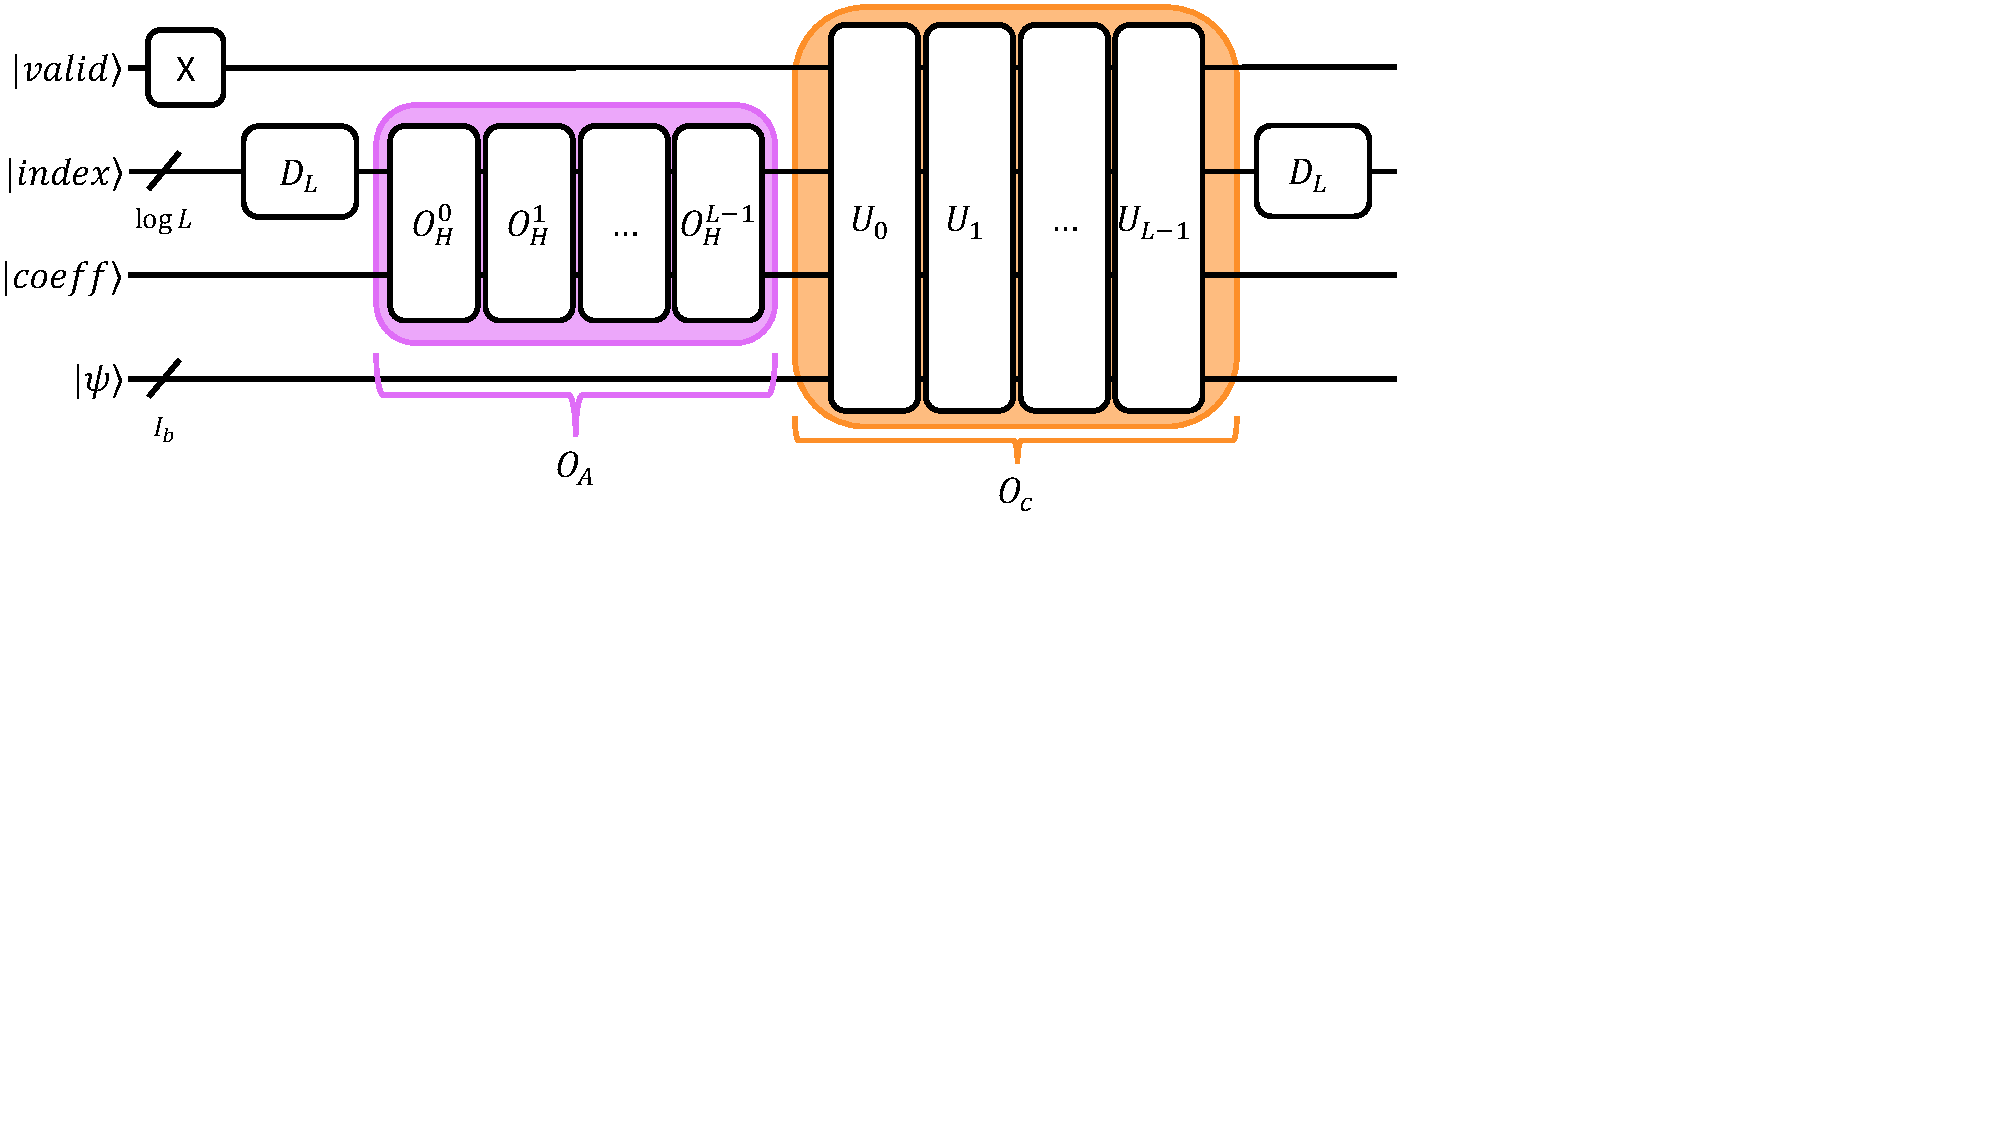
\includegraphics[width=12cm]{figures/liu-construction.pdf}
    \caption{
        \textbf{Sparse-Oracle Block-Encoding Circuit for Pairing Hamiltonians}
        A circuit diagram for the block-encoding described by Liu et. al \cite{liu2024efficient} is shown.
        The $O_A$ oracle is implemented by the series of $O_H^l$ operators (shaded in purple) which load the coefficients of the $l^{th}$ term.
        The $O_c$ oracle is implemented by the series of $U_l$ operators (shaded in orange) which apply the $l^{th}$ term onto the state.
        The $D_L$ oracle represents the diffusion operator (Eq. \ref{eq:diffusion-had}) acting on $L$ terms where $L$ is raised to the nearest power of two.
        The unitary $U_H = D_L O_c O_A D_L$ implements a block-encoding of the pairing Hamiltonian (Eq. \ref{eq:pairing-ham}) assuming the validation qubit ($\ket{\text{valid}}$) is initialized in the $\ket{1}$ state.
        The rescaling factor of this block encoding is given by $\lambda = L \max_{ij} {|h_{ij}|}$.
    }
    \label{fig:liu-construction}
\end{figure}

\begin{figure}[h]
    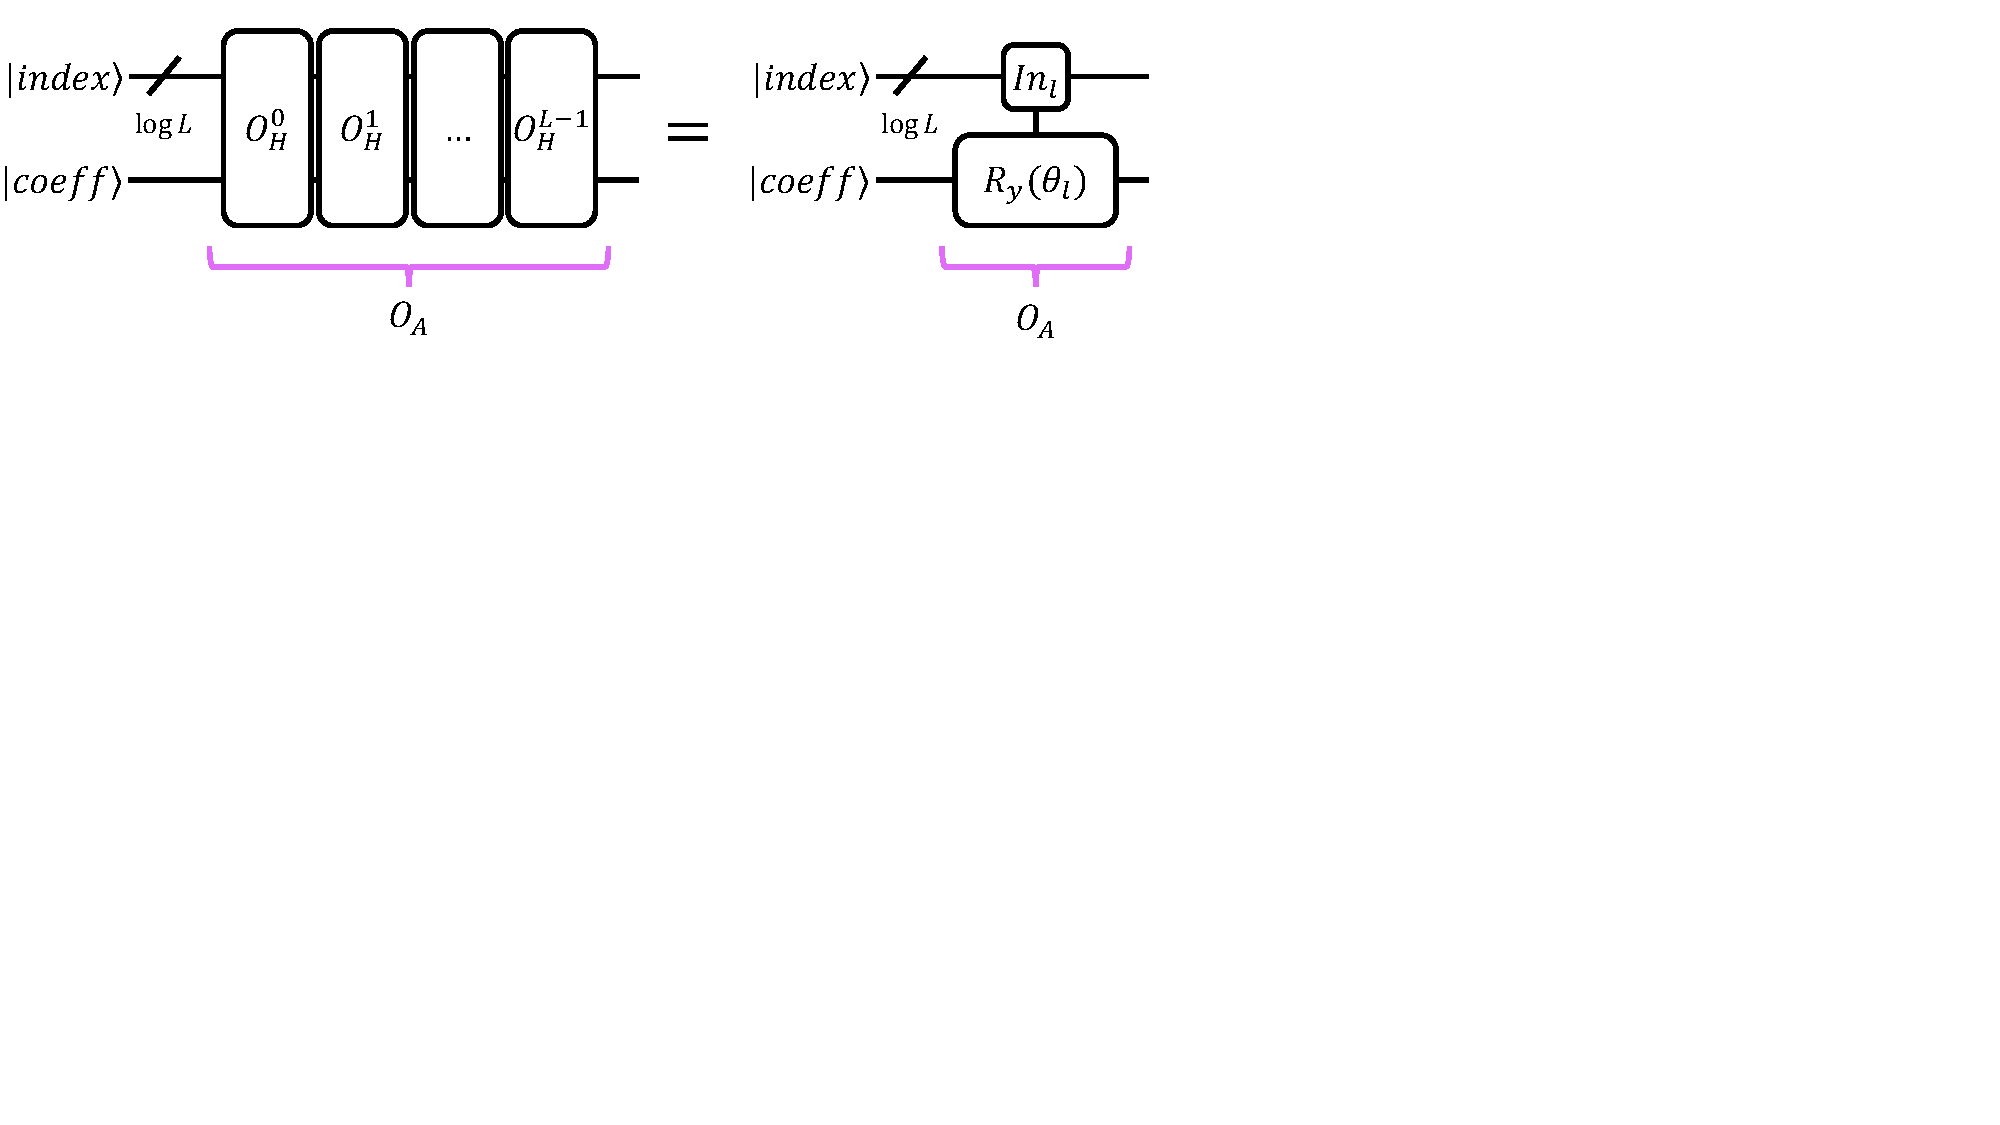
\includegraphics[width=12cm]{figures/liu-O_A.pdf}
    \caption{
        \textbf{$O_A$ Circuit for Pairing Hamiltonians}
        A circuit diagram for the $O_A$ oracle described by Liu et. al \cite{liu2024efficient}.
        Each unitary in the subfigure on the left performs an $R_y$ rotation on the coefficient qubit, controlled on the index register being in the computational basis state $\ket{l}$.
        This sequence of controlled rotations is referred to as a set of uniformly controlled rotations which is depicted by the subfigure on the right.
        Further discussion of compiling uniformly controlled rotations is given in Appendix \ref{sec:multiplexed-rotations}.
    }
    \label{fig:liu-O_A}
\end{figure}

Following Eq. \ref{eq:value-oracle}, each $O_H^l$ oracle rotates an ancilla qubit ($\ket{\text{coeff}}$ in Figure \ref{fig:liu-construction}) proportionally to the coefficient of the $l^\text{th}$ term when the index register ($\ket{\text{index}}$) is in the computational basis state $\ket{l}$.
This can be achieved by an $R_y$ rotation:
\begin{equation}
    \begin{split}
        & R_y (\theta_l) \ket{0}_\text{coeff} = h_{ij} \ket{0}_\text{coeff} + \sqrt{1 - |h_{ij}|^2} \ket{1}_\text{coeff} \\
        & \theta_l = 2 \cos^{-1}{(h_{ij})}
    \end{split}
\end{equation}
where the rotation is controlled on the index register being in the $l^\text{th}$ computational basis state.
This sequence of rotations controlled on the basis states of the index register is sometimes referred to as a set of uniformly controlled rotations.
The construction given by Möttönen et. al \cite{mottonen2004transformation} for uniformly controlled rotations results in the $O_A$ oracle using $L$ uncontrolled rotations.
A further discussion of this compilation is given in Appendix \ref{sec:multiplexed-rotations}.

The $O_c$ oracle is constructed by the series of unitaries denoted as $U_0 \dots U_{L - 1}$ in Figure \ref{fig:liu-construction}.
Similar to the $O_H^l$ unitaries, each $U_l$ unitary is controlled on the index register being in the computational basis state $\ket{l}$.

The controls on the index register for each $U_l$ comprising the $O_c$ oracle ensure that only the $l^\text{th}$ term is applied when the computational basis state is in the $\ket{l}$ state.
These controls on the index register are present for each term and can be accounted for by the uniformly controlled operation structure discussed in more detail in Appendix \ref{sec:uniformly-controlled-operations}.

\begin{figure}[h]
    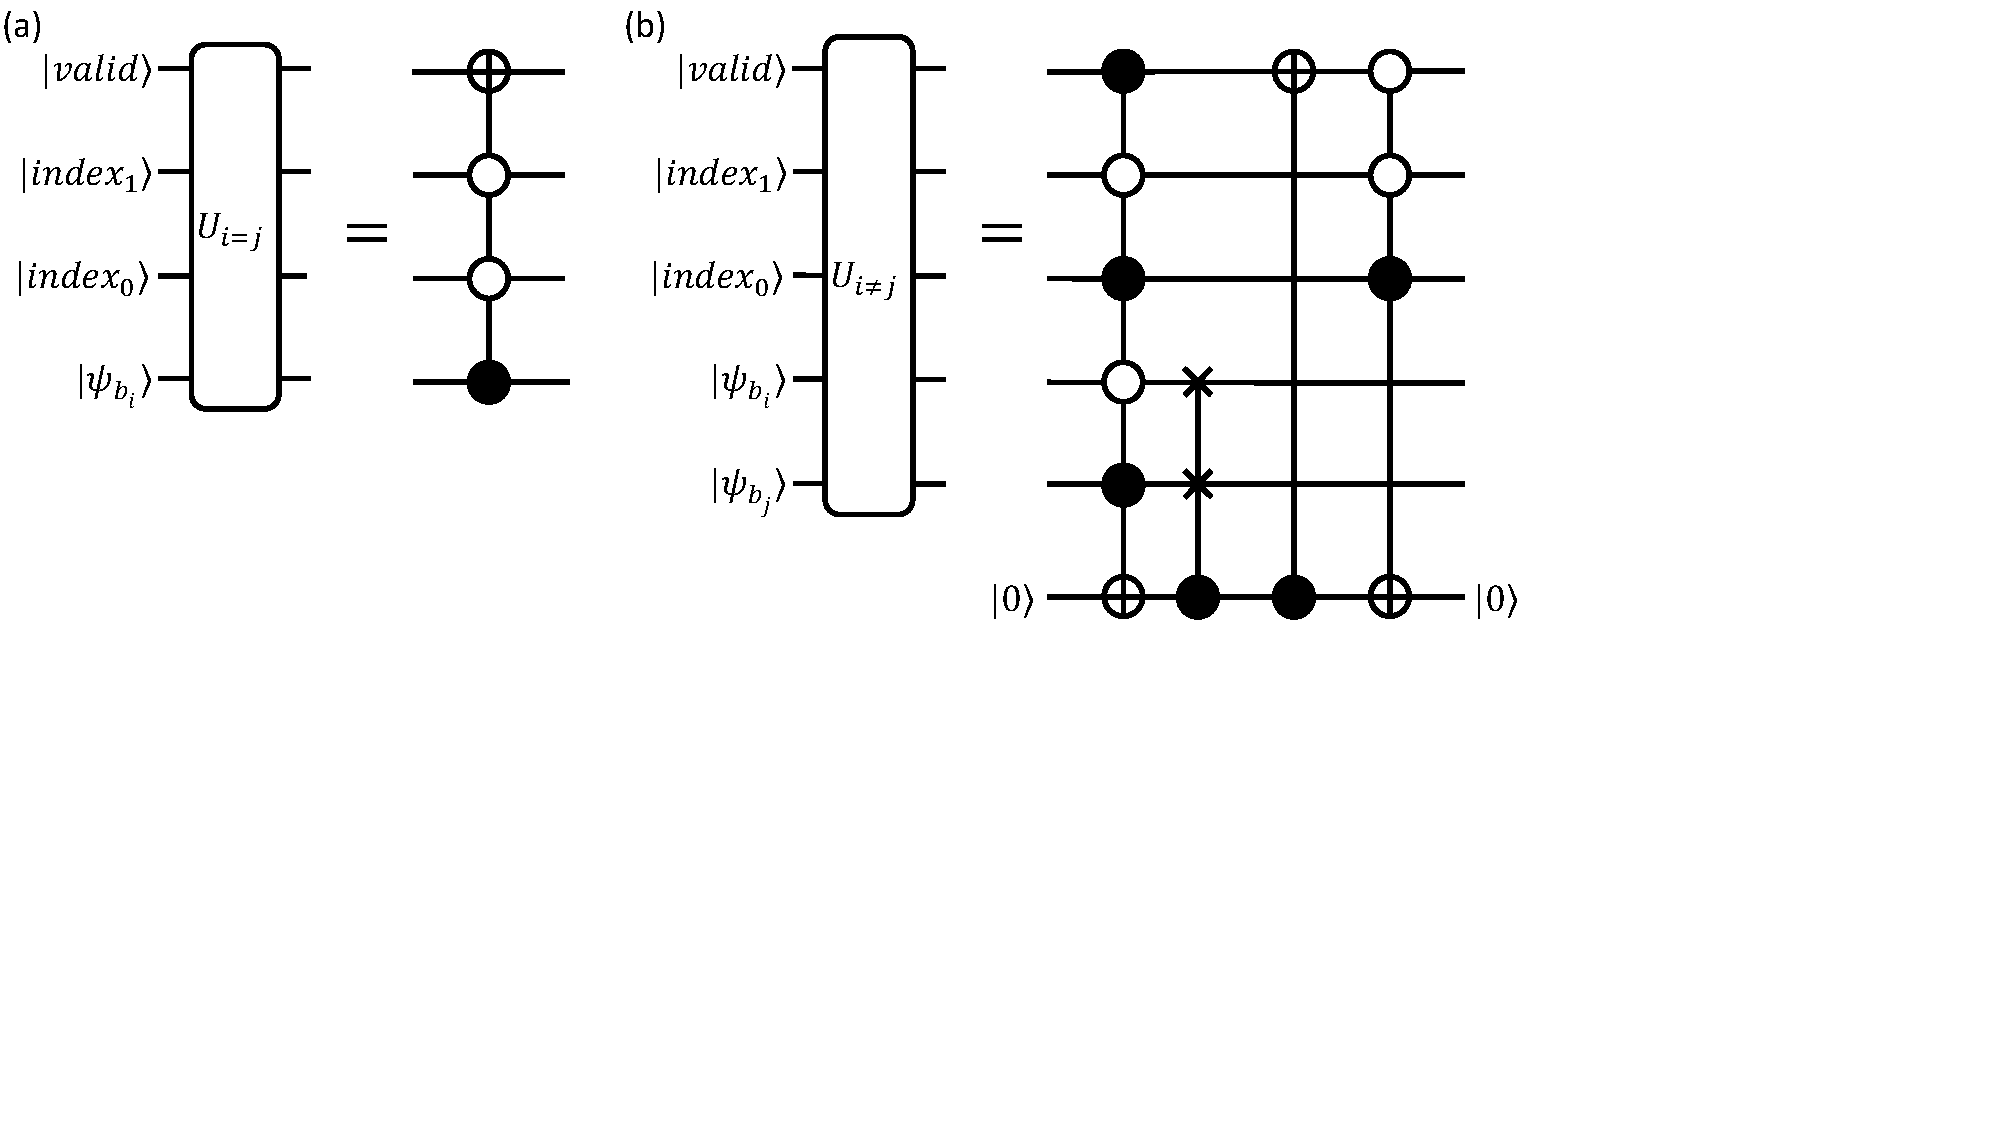
\includegraphics[width=12cm]{figures/liu-O_c.pdf}
    \caption{
        \textbf{$O_c$ Circuit Components for Pairing Hamiltonians}
        A circuit diagram for the unitaries comprising the $O_c$ oracle described by Liu et. al \cite{liu2024efficient} are shown.
        The circuit in subfigure a shows the unitary $U_{i = j}$ which applies a block-encoding of the operator $b_i^\dagger b_i$ when the index register is in the computational basis state $\ket{0}$. 
        The circuit in subfigure a shows the unitary $U_{i \neq j}$ which applies a block-encoding of the operator $b_i^\dagger b_j$ when the index register is in the computational basis state $\ket{1}$.
        The validation qubit ($\ket{\text{valid}}$) is assumed to begin in the $\ket{1}$ state.
    }
    \label{fig:liu-O_c}
\end{figure}

Liu et. al give constructions for applying the terms in the pairing Hamiltonian onto the system under the two cases $i = j$ and $i \neq j$.
When the index for the ladder operators in Eq. \ref{eq:pairing-ham} are the same ($i = j$), the operator $b_i^\dagger b_i$ should zero-out the quantum state when the $i^\text{th}$ mode is unoccupied and should leave the state unchanged when the mode is occupied. 
For these terms, the desired action is for the validation qubit to end in the $\ket{1}$ state if the mode is unoccupied and end in the $\ket{0}$ state if the mode is occupied.
This can be achieved by a Toffoli gate which is controlled on the $i^\text{th}$ mode being occupied and the index register being in the computational basis state $\ket{l}$, assuming the validation qubit is initialized in the $\ket{1}$ state.
A circuit diagram for this block-encoding is given in Figure 11 of \cite{liu2024efficient} and we give a reproduction in Figure \ref{fig:liu-O_c}a.

When the indices that the ladder operators act on are not the same ($i \neq j$), the operator $b_i^\dagger b_j$ should zero-out the quantum state \textit{unless} both the $i^\text{th}$ mode is unoccupied \textit{and} the $j^\text{th}$ mode is occupied.
Otherwise, the system of the state would be zeroed-out which would be indicated by the validation qubit being in the $\ket{1}$ state.
If these conditions are true, a swap gate can be applied to swap the occupations of the fermionic modes and the validation qubit is flipped to the $\ket{0}$ state. 

To perform this action, an ancilla qubit can be used to store the logical-AND of the conditions on the validation qubit, the index register, and the occupation states of the fermionic modes.
We assume that this ancilla qubit begins in the $\ket{0}$ state and the intent will be to return it to the $\ket{0}$ state such that it can be reused on subsequent operations.
In this work, we refer to qubits that are only temporarily rotated outside of the $\ket{0}$ state, but are returned to the $\ket{0}$ state at the end of an operation as clean ancillae.
An example for a circuit to perform this operation is given in Figure 11 of \cite{liu2024efficient} and we give a reproduction in Figure \ref{fig:liu-O_c}b.
We note that to properly uncompute the ancilla qubit and return it to the $\ket{0}$ state we include the controls on the index register.
These controls are not present in the constructions given by Liu et. al, but must be included to properly reset this ancilla qubit.
\ws{Determine if construction by Liu et. al is actually incorrect or just incorrect if you want to treat the ancilla qubit as a clean ancilla.}
